\documentclass{article}

\usepackage{color}
\usepackage{graphicx}
\usepackage{tabularx}
\usepackage[frenchb]{babel}
\usepackage[utf8]{inputenc}
\usepackage[T1]{fontenc}
\usepackage{lmodern}

\usepackage{geometry,wrapfig,lipsum}
 \geometry{
 top=20mm,
 bottom=20mm,
 }


\title{Hacking}
\author{Justal Kevin}
\date{30/10/2015}
\renewcommand{\contentsname}{Table des mati\`eres} 
 
\newcommand\invisiblesection[1]{%
  \refstepcounter{section}%
  \addcontentsline{toc}{section}{\protect\numberline{\thesection}#1}%
  \sectionmark{#1}} 
 
\begin{document}

\begin{center}
\textbf{\Huge{STICKY WALL}}\\
\line(1,0){300}\\
Projet de CEIHM\\
\vspace{3cm}
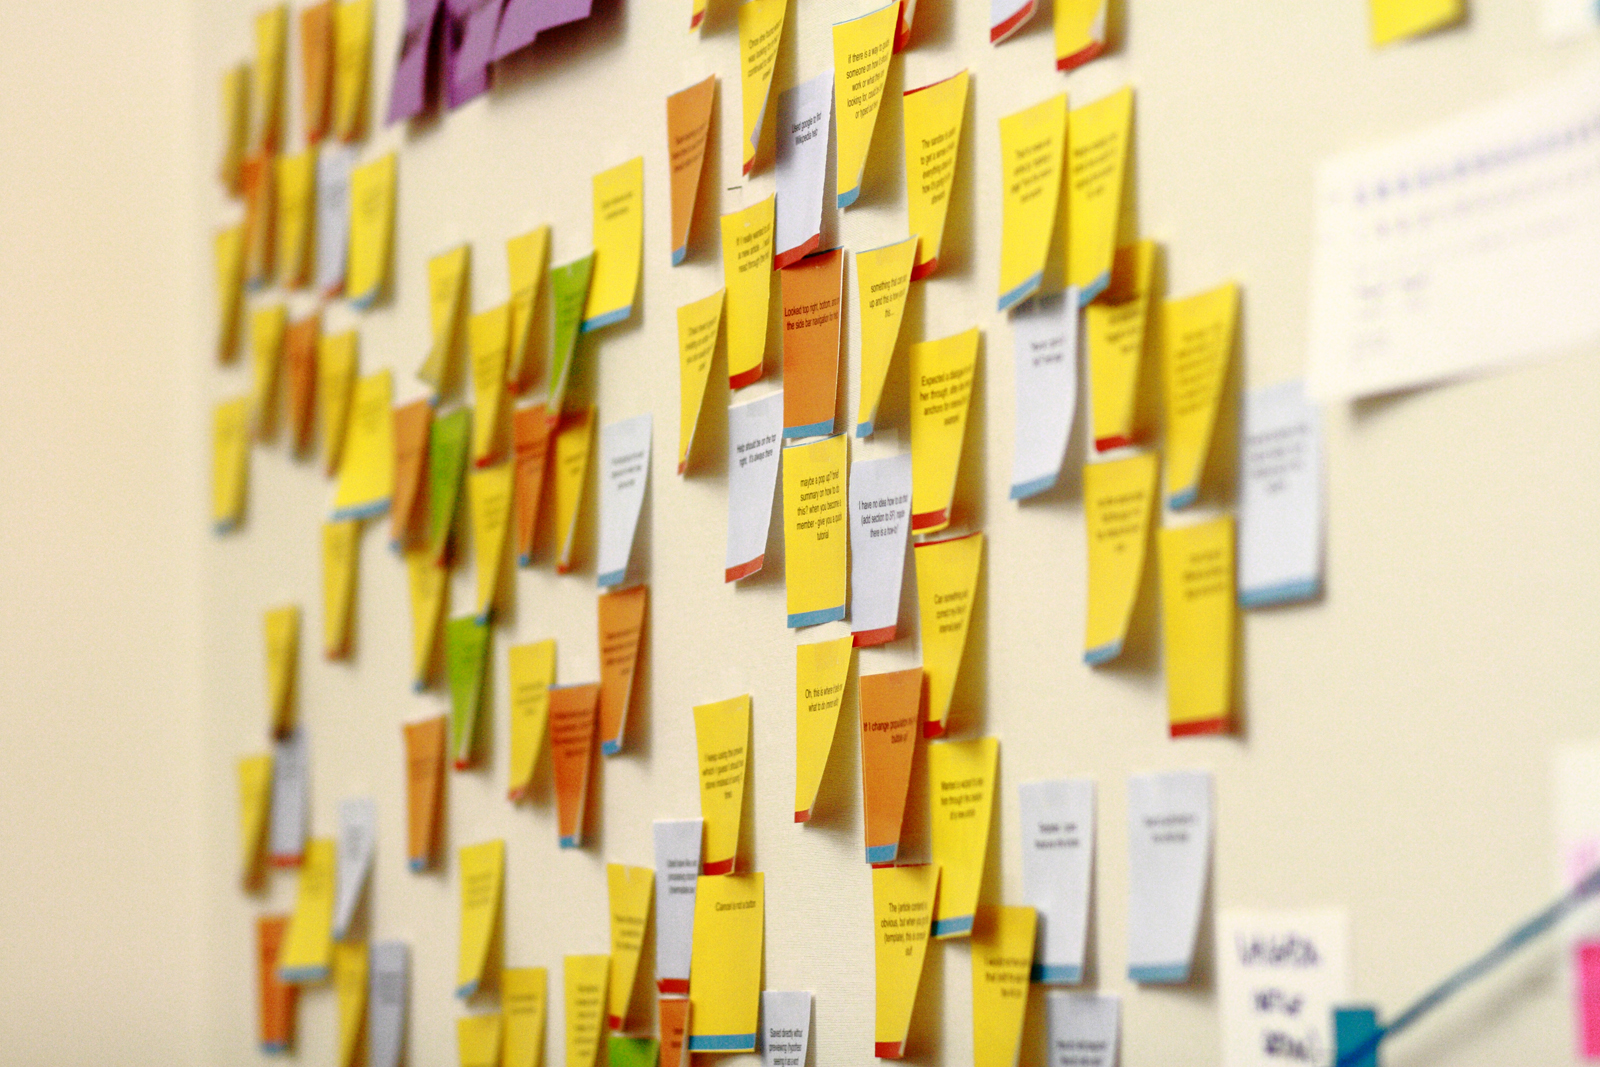
\includegraphics[width=\textwidth]{1}\\
\vspace{3cm}
2015-2016\\
\vspace{4.5cm}
\textbf{Justal Kevin - \color{blue}{\underline{justal.kevin@gmail.com}}}\\
\textbf{Isoard Jean-Christophe - \color{blue}{\underline{jeanchristophe.isoard@polytech.unice.fr}}}\\
\textbf{Kha Jean-phillipe - \color{blue}{\underline{kha.jp@polytech.unice.com}}}\\
\end{center}

\newpage
\tableofcontents

\newpage
\section{Analyse de l'existant}
\subsection{Compréhension initiale du sujet}
\hspace*{0.6cm}Le but du sujet est de réaliser une assistance pour un sticky wall permettant de réaliser électroniquement ce que l'on attend d'un sticky wall murale mais sans les inconvénients lié à ce dernier. C'est à dire d'avoir un jeu de post-it sans être limité par le format d'une feuille de papier, par le matériel et par les conditions de la pièce où repose le sticky wall. Il faut donc que le sticky wall électronique permettent d'ajouter, de supprimer, de déplacer des post-it tout en les sauvegardant pour pouvoir récupérer le travail effectué d'où l'on souhaite. Il faut de plus que ce dernier permette de connecter plusieurs utilisateurs simultanément sur le sticky wall pour que les différents utilisateurs qui peuvent être éparpillé sur la planete travaille ensemble sur le même document. Ce genre de sticky wall s'adresse en particulier au groupes de travail. C'est à dire à des groupes qui demandent de la synchronisation et ou du travail de reflexion collectif tel des développeurs, facilitateurs... Ces personnes ont généralement besoin d'exprimer leurs idées aux autres pour que le groupe puisse ensuite en discuter ou de dire sur quelle tâches ils travaillent actuellement pour éviter que deux personnes travaille sur la même tâche.
\subsection{Recensement de dispositifs (interfaces) plus au moins similaires au dispositif (interfaces) à concevoir dans le mini-projet}
\hspace*{0.6cm}De nombreux sites sur Internet permettent de créer des sticky wall. Cependant aucun d'eux ne réalise vraiment ce que l'on attend d'un tel dispositif. Dans les plus connus, on peux noter :\\

\textbf{stormboard.com}
\vspace{0.2cm}\\
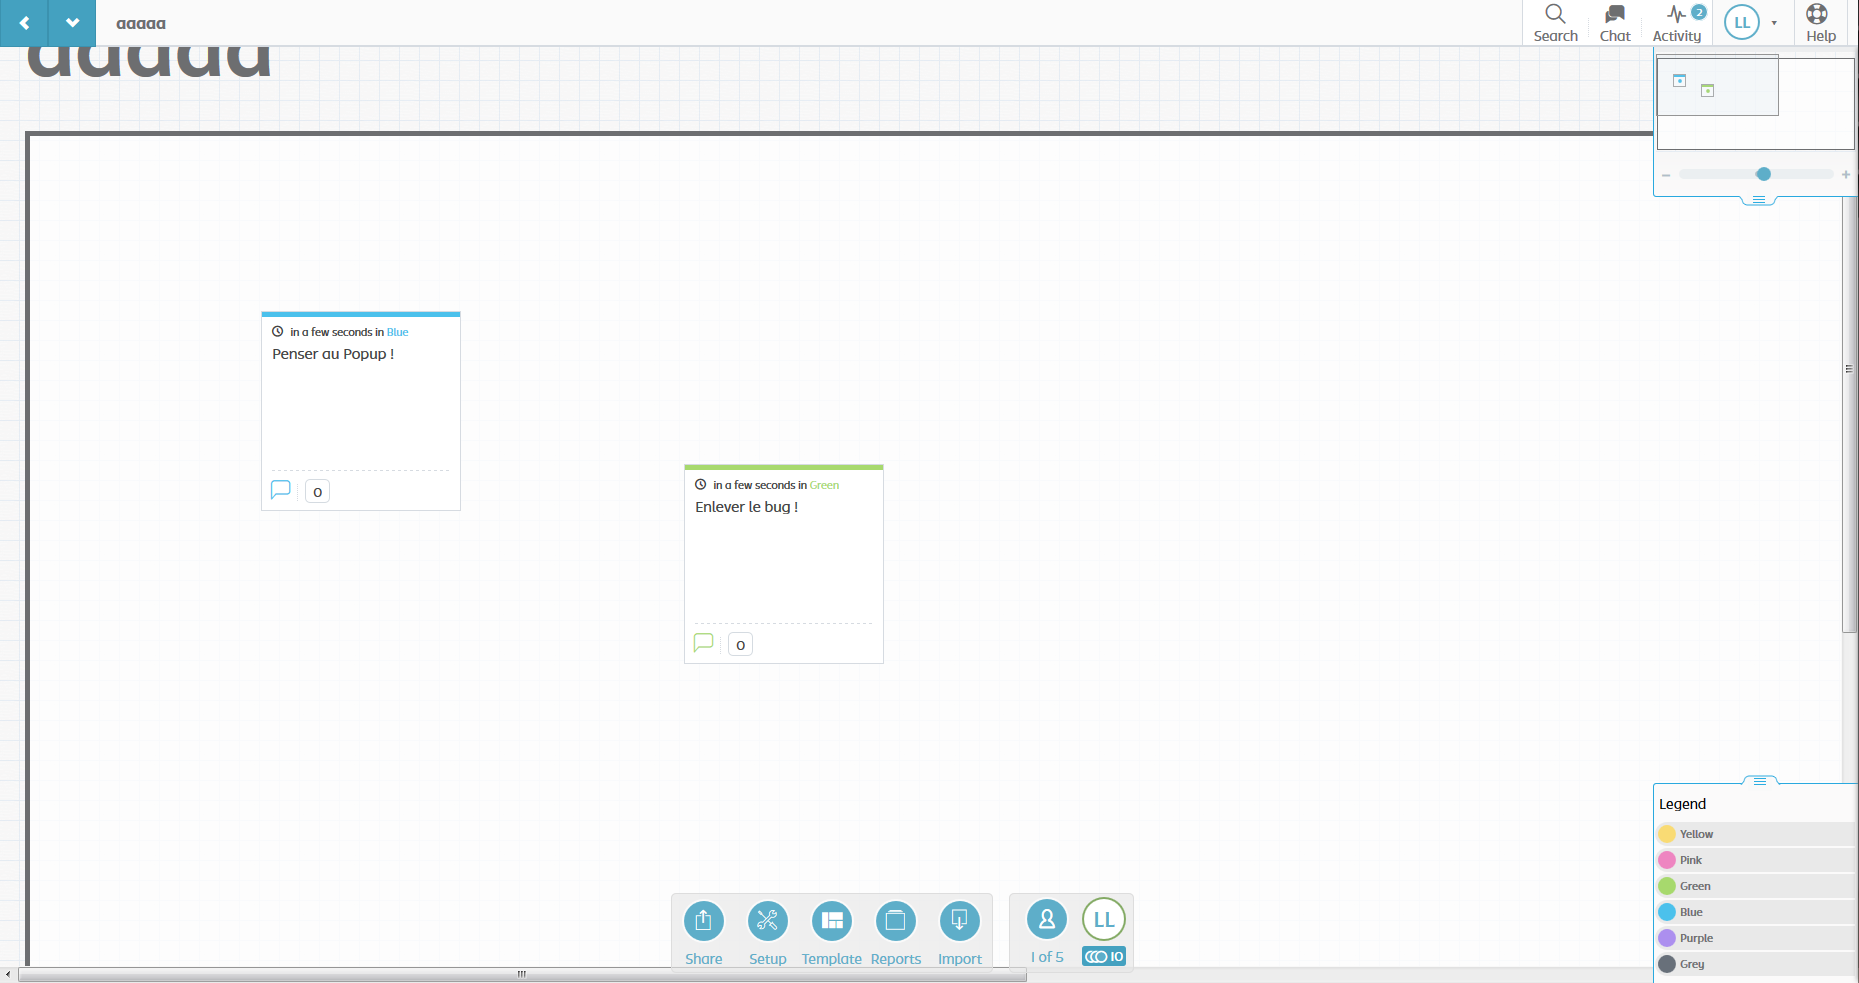
\includegraphics[width=\textwidth]{2}\\
\vspace{0.2cm}\\
Cette application en ligne présente de nombreux avantages :
\begin{itemize}
  \item Il n'y a pas de limite au mur
  \item On peux travailler à plusieurs sur le même mur et ce sur toutes la planète
  \item Il est possible de faire des post-its de différentes tailles
  \item On peux inclure des médias comme des vidéos ou images
  \item Historique d'activités
\end{itemize}
\vspace{0.2cm}
\hspace*{0.6cm}Cependant, on dénote et regrette que l'application ne dispose pas d'un système de grille permettant de faire de grosse séparation entre les post-it et ainsi les trier par leurs avancements. On regrette aussi que cette application ne dispose pas d'un outil pour créer différents moyen de relier les post-it entre eux (avec des flèches de différentes tailles, différentes couleurs...).
\vspace{0.2cm}\\
\textbf{Walfle}
\vspace{0.2cm}\\
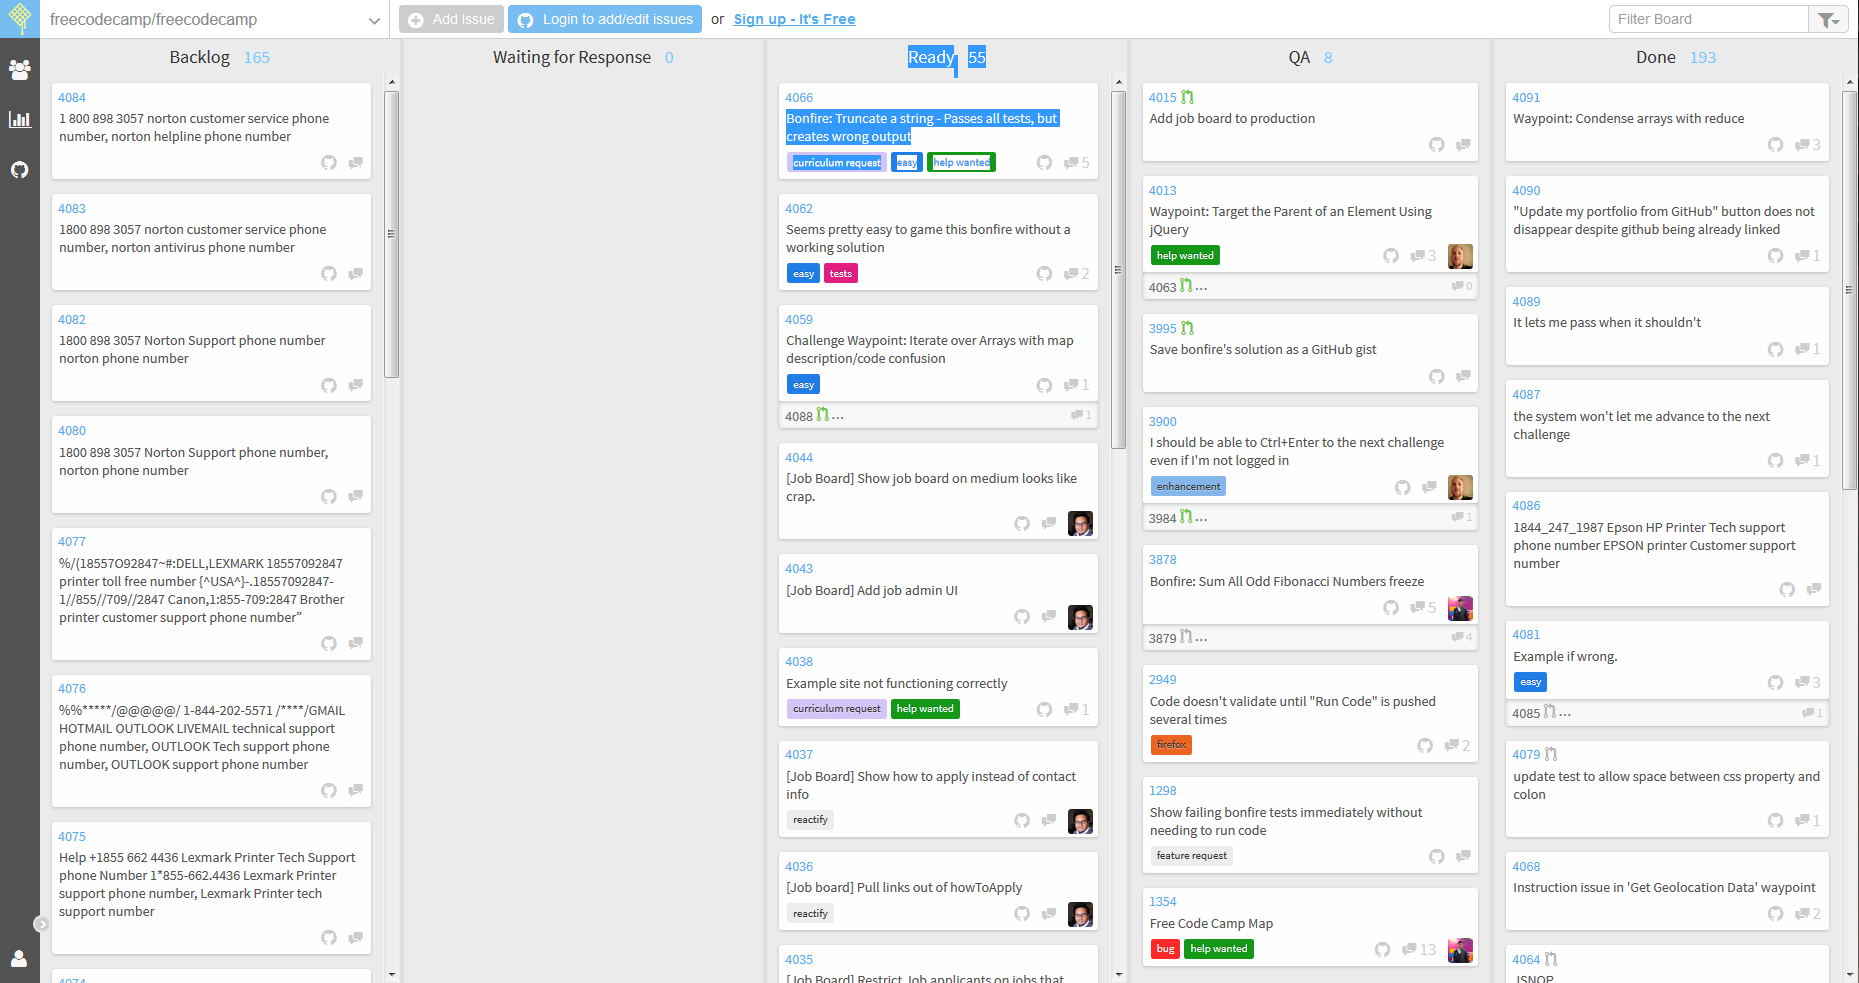
\includegraphics[width=\textwidth]{4}\\
\vspace{0.2cm}\\
Encore une application en ligne :
\begin{itemize}
  \item On peux travailler à plusieurs sur le même mur et ce sur toutes la planète
  \item Les post sont affecté
  \item Colonnes de séparation
  \item Historique d'activités
\end{itemize}
\vspace{0.2cm}
\hspace*{0.6cm}Cependant, sur ce wall on regrette de ne pas pouvoir ajouter des médias ou encore de pouvoir dézoomer pour afficher l'ensemble du mur.
\vspace{0.2cm}\\
\textbf{Sticky wall manuel}
\vspace{0.2cm}\\
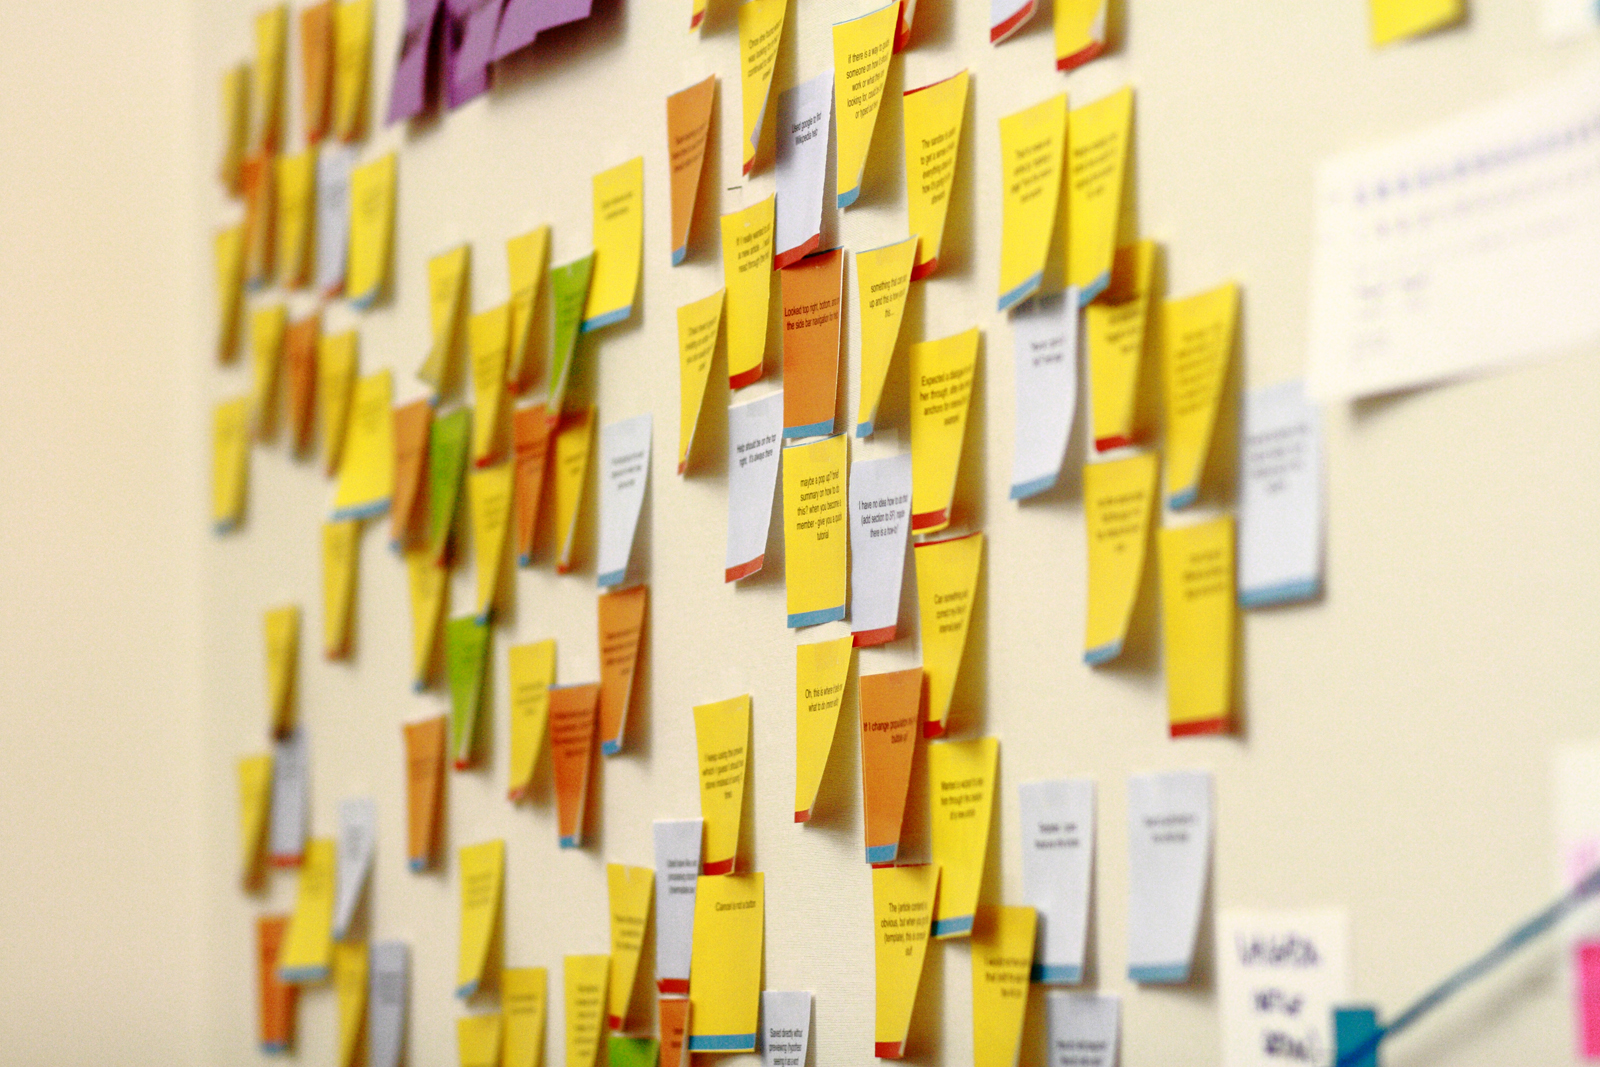
\includegraphics[width=\textwidth]{1}\\
\vspace{0.2cm}\\
Il s'agit du sticky wall de base, cette version manuel est ce que l'on veut informatiser. Comme les autres dispositifs et/ou interfaces, ce dernier possède la aussi des avantages :
\vspace{0.2cm}\\
Cette application en ligne présente de nombreux avantages :
\begin{itemize}
  \item Facile à mettre en place
  \item Hors-ligne (il n'y a donc pas besoin d'internet)
  \item Collaboration à plusieurs simultanément
\end{itemize}
\vspace{0.2cm}
\hspace*{0.6cm}Cependant là encore, il y a des inconvénients. Qui dit manuel, dit qu'il faut le matériel nécessaire. Il faut pour ce sticky wall des post-its vierge en grand nombre. Il seront de plus jeté lorsque le wall ne servira plus (écologie ?). Ce wall est difficilement déplaçable si ce dernier est relativement grand. On ne peux travailler avec des gens de divers pays en même temps à moins d'utiliser une caméra et de filmer. Il faut créer sois même un système d'historisation avec une caméra. Et enfin, c'est un système qui repose sur de la colle, si la pièce est à une température un peu élevé ou si le mur est posé depuis plusieurs semaines, des post-its ainsi que le mur entier peut tomber et s'écrouler.

\subsection{Recensement des types d’utilisateurs à qui ces dispositifs existants sont ou étaient destinés}
\hspace*{0.6cm}Ces dispositifs sont destinées globalement à toutes personnes voulant effectuer quelques choses à plusieurs. Pour être plus précis, nous allons voir cela sous forme de liste :
\vspace{0.2cm}
\begin{itemize}
  \item \textbf{Les développeurs} : Il s'agit là d'un des groupes phares qui utilise très souvent un sticky wall. On peux dès lors donner un exemple : \textit{https://waffle.io/freecodecamp/freecodecamp}\\
Pour le free code camp, des développeurs du monde entier travaille sur le même projet, il apparait donc important pour ces derniers d'avoir une manière de voir qui travaille sur quoi afin de ne pas faire deux fois la même chose.
  \item \textbf{Les facilitateurs} : Ce groupe de personnes sont les clés d'un bon groupe. Ils travaillent régulièrement avec des groupes de divers horizons et se servent très souvent de Sticky wall pour receuillir les informations de chacun pour faire avancé un débat ou un projet.
  \item \textbf{Les businessmans} : Ce groupe de personnes se servent souvent d'un stiky wall pour faire un brainstorming et recenser sur un tableau l'ensemble des idée des gens dans une réunion.
  \item {Les autres} : Un sticky wall est finalement utile pour toutes personnes voulant effectué un travail en groupe et avoir l'ensemble du projet sous les yeux, les étudiants, les chefs de projet...
\end{itemize}
\subsection{Recensement des besoins/buts des types d’utilisateurs, en rapport avec les dispositifs existants}
\hspace*{0.6cm}Cette partie reprend un peu ce qui a déjà été dit. Dans les dispositifs existants, les différents utilisateurs recherchent les buts ou besoins suivants :
\vspace{0.2cm}
\begin{itemize}
  \item \textbf{Exposition du projet} : pouvoir voir instantanément l'ensemble du projet
  \item \textbf{Avancement du projet} : pouvoir voir instantanément l'état actuel du projet
  \item \textbf{Synchronisation} : pouvoir synchroniser des personnes sur un travail collectif
  \item \textbf{Brainstorming} : pouvoir afficher l'ensemble des idées d'un groupe de personnes et faire participer un grand nombre de personnes simultanément
  \item \textbf{Vitesse d'avancement du projet} : pouvoir à partir de l'historique du sticky wall prévoir le temps pour finaliser le projet
\end{itemize}
\subsection{Recensement des tâches utilisateurs que les dispositifs existants sont censés satisfaire}
\hspace*{0.6cm}Tous les dispositifs ne se valent pas, certaines ont certaines fonctionnalités très pratiques que d'autres n'ont pas. Ci-dessous se trouvent la liste des différentes tâches que les dispositifs existants satisfassent :
\vspace{0.2cm}
\begin{itemize}
  \item Ajout de post-it
  \item Redimensionnement de post-it
  \item Création de colonne de séparation sur le sticky wall
  \item Ajout de différentes couleurs sur les post-it
  \item Déplacement des post-it
  \item Connexion entre les post-it
  \item Ajout de média dans les post-it
  \item Suppresion de post-it
  \item Cloturer un post-it
  \item Affecter un post-it
  \item Agrandir le sticky wall
  \item Sauvegarder le sticky wall
  \item Partager le sticky wall
  \item Activité simultané par plusieurs utilisateurs sur le sticky wall
\end{itemize}
\subsection{Recensement des scénarios utilisateurs associés aux dispositifs existants}
\hspace*{0.6cm}Dans la pratique, il y une infinité de scénarios possibles mais on peux ressortir les plus globaux :
\vspace{0.2cm}\\
Nous sommes dans le contexte suivant : nous effectuons un brainstorming avec plusieurs personnes
\begin{itemize}
  \item L'utilisateur a une idée
  \item L'utilisateur créer son post-it
  \item L'utilisateur le met sur le mur
  \item L'ensemble des personnes peuvent alors voir ce post-it
\end{itemize}
\vspace{0.2cm}
Imaginons maintenant que nous travaillons à plusieurs sur un projet
\begin{itemize}
  \item L'utilisateur regarde les post-it dans la premiere colonne (à gauche)
  \item L'utilisateur s'affecte le post-it
  \item L'utilisateur le déplace alors dans la colonne à droite pour dire qu'il travaille actuellement dessus
  \item L'utilisateur le déplace alors à droite pour dire qu'il a fini sa tâche
  \item Le post-it est alors archivé ou rentre alors dans une nouvelle phase suivant le sticky wall (phase de test effectué par d'autre utilisateur...)
\end{itemize}
\vspace{0.2cm}
Imaginons maintenant que nous voulons organiser un projet
\begin{itemize}
  \item L'utilisateur analyse avec d'autres personnes les post-it
  \item Le facilitateur réorganise les post-it en les déplaçant et en effectuant des liens (flèches) entre les différents post-it.
  \item Puis le groupe de personne rediscute de l'organisation actuelle des post-it jusqu'à un tableau final qui sera l'organisation et l'ordre dans lequel les tâche seront effectué.
\end{itemize}
\subsection{Recensement des problèmes éventuels rencontrés pas les utilisateurs des dispositifs existants}
\hspace*{0.6cm}Les problèmes rencontrés par les utilisateurs sont surtout axé sur la manipulation et sur la compréhension du système. Après avoir fait testé quelques personnes sur ces divers dispositifs, on a vite remarqué que de mauvais choix sur l'interface graphique ou sur le comportement de l'application rendent cette dernière compliqué à utiliser. Par exemple :
\vspace{0.2cm}
Imaginons maintenant que nous voulons organiser un projet
\begin{itemize}
  \item Il n'est pas naturel de faire double-clic pour créer un post-it quand il y a un bouton pour en ajouter un en base
  \item Il n'est pas naturel non plus de déplacer un post-it avec le clic droit
  \item Il faut d'abord choisir la couleur du post-it avant de le créer car on ne peux pas la changer pendant la création du post-it
  \item Un wall infini dès le départ perd l'utilisateur
  \item Si il n'y a plus internet, on peux continué à utiliser le wall mais celui-ci n'est pas sauvegardé sur le serveur.
\end{itemize}

\section{Personnas}
\subsection{Les développeurs}
\begin{wrapfigure}{l}{0.4\textwidth}
  \vspace{-20pt}
  \begin{center}
    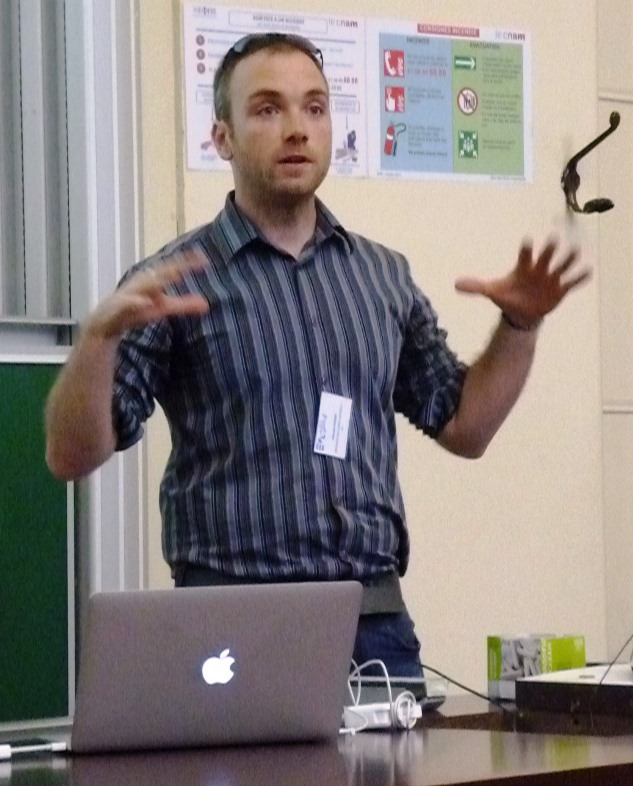
\includegraphics[width=0.37\textwidth]{Mosser}
  \end{center}
  \vspace{-20pt}
  \vspace{-10pt}
\end{wrapfigure}
\textbf{Sébastien Mosser}
\vspace{0.2cm}\\
\underline{Age}: 31 ans
\vspace{0.2cm}\\
\underline{Profession} : Maître de conférence
\vspace{0.2cm}\\
\underline{Relation à la technologie} : 10/10 C'est son métier
\vspace{0.2cm}\\
\underline{Utilisation d'un sticky wall} : Oui
\vspace{0.2cm}\\
\underline{Verbatim} : Il faut que ce soit simple et rapide. On ne doit pas se battre avec la technologie.
\vspace{0.2cm}\\
\underline{Caractéristiques}
\begin{itemize}
  \item N'aime pas gaspiller son temps
  \item Aime la simplicité
\end{itemize}
\vspace{0.2cm}
\underline{Besoins}
\begin{itemize}
  \item Collaboration
  \item Échanger des idées
\end{itemize}
\hfill\\
\vspace{-1cm}\\

\hfill\\
\textbf{Objectifs}
\begin{itemize}
  \item Simplifier l'utilisation
  \item Augmenter la vitesse d'installation
  \item Partager d'informations
  \item Travailler à plusieurs simultanément
  \item Réutiliser le mur
  \item Déplacer des post-it
  \item Pouvoir voir l'avancer d'un projet
  \item Pouvoir envoyer des images
  \item Manipuler le contenu post-it
\end{itemize}
\vspace{0.2cm}
\textbf{Chemin vers l'objectifs}
\begin{itemize}
  \item Un simple lien ou simple bouton permet de créer ou d'ouvrir un nouveau wall
  \item Affichage sur un grand mur (projecteur,écran...)
  \item Via un bouton, je peux sauvegarder l'état actuel du mur
  \item Je prend une photo avec mon portable et je l'envoie sur mon mur dans un post-it via une application.
  \item Je prends le post-it et je le met à l'endroit où je le lâche. Pour la sélection, il faut que ce soit évident et simple, comme un pointeur avec une wiimote.
  \item Avec un bouton, je peux superposer mon wall actuel avec celui du date antérieur (en selectionannt une date dans une option)
  \item Un bouton permet d'ajouter une image en piece jointe
  \item Un bouton permet de dessiner sur un post-it
  \item Je redimensionne en prenant le coin de mon post-it puis je l'étire ou le réduit.
  \item Je peux faire des zone sur mon tableau en faisant un glisser dans une zone vide du wall.
\end{itemize}
\vspace{0.2cm}
\textbf{Objections}
\begin{itemize}
  \item Verouillage ou protection sur les post-it
  \item Déplacer les post-it avec un accessoire lourd (comme un téléphone)
  \item Trop complexe
  \item Trop de fonctions inutiles
\end{itemize}
\vspace{0.2cm}
\textbf{Commentaires}
\begin{itemize}
  \item Pourquoi ne pas mettre des tags ?
\end{itemize}
\subsection{Les facilitateurs ?}

\section{Scénario de notre maquette}

\subsection{Le BrainStorming}
\subsubsection{Description de l’activité}
Imaginons une réunion entre plusieurs personnes. Le facilitateur pose une question à l'ensemble des personnes présente. Chacune des personnes présente créer alors de petit post-it électronique avec une tablettes ou téléphones et les envoies sur le mur en utilisant une connections quelconque comme Internet ou Bluethooth.
\subsubsection{Spécification de l’utilisateur}
Un facilitateur est une personne qui sont chargé de coordonner plusieurs personnes au sein d'un groupe afin que le travail soit efficace et prenne le maximum de toutes les personnes présentes.
\subsubsection{Résultat attendu}
Recueillir l'ensemble des post-it créer par chacune des personnes sur un sticky wall.
\subsubsection{Circonstances}
Le facilitateur doit réussir à faire participer l'ensemble des personnes sans donner trop de voix à quelqu'un en particulier. Avec des post-it et un wall, chacune des personne ont leurs mots à dire et celui-ci à pour chacun la même importance.

\subsection{Le maniement d'un post-it}
\subsubsection{Description de l’activité}
Imaginons nous arriver dans un projet en cours avec X personnes. Il y a 3 colonnes sur le sticky wall electronique. La première est la colonne avec les post-it représentant les tâches à accomplir, la seconde représente les tâches en cours de réalisation et la dernière les tâches effectués. Nous allons dans un premier temps, nous affecter un post-it (avec un champ) et le déplacer sur la colonne en cours de traitement via notre téléphone ou notre tablette. Plus tard dans la journée, trouvant que la tache est beaucoup plus importante que prévu dans l'application, on se décide de revenir sur le sticky wall et d'agrandir la tache pour bien montrer que celle-ci occupe une place importante, on décide aussi de la changer de couleur. Une fois que nous avons fini la tache, on la déplace ensuite dans la 3ieme colonne.
\subsubsection{Spécification de l’utilisateur}
Un collaborateur est une personne qui participe à un projet et qui doit effectuer différentes tâche dans la journée en fonction du sticky wall.
\subsubsection{Résultat attendu}
Pouvoir manier et éditer des post-it
\subsubsection{Circonstances}
Le développeur ou le collaborateur dans le projet doit pouvoir agir sur les post-it afin de faire transparaitre sur quoi il travaille et de le faire savoir aux autres membres du groupe de travail.

\subsection{L'injection de médias}
\subsubsection{Description de l’activité}
Alors que nous sommes entrain de participer activement sur un projet à plusieurs, on prend un livre en rapport avec notre travail et tombons sur un article très intéressant pour notre travail et l'on souhaite le faire partager sur le sticky wall. On prend alors notre téléphone afin de prendre une photo de cet article. Une fois fait, on envoie la photo directement sur le mur via notre téléphone.
\subsubsection{Résultat attendu}
Pouvoir envoyer des photos sur le sticky wall
\subsubsection{Circonstances}
Toutes personnes travaillant sur le sticky wall doit pouvoir envoyer sur le mur des photos afin de partager une informations jugé utile pour les autres.

\subsection{Les liaisons}
\subsubsection{Description de l’activité}
Nous sommes lors d'une réunion avec un groupe de personnes, il y sur un mur un ensemble de post-it. En fonction des discutions avec les différentes personnes, nous allons analyser les relations entre les post-it. Tout en faisant cela, on relie les post-it les uns avec les autres en selectionant l'outil pour relier les post-it. On choisit ensuite le type de liasons que l'on souhaite faire dans la fenetre de droite puis on selectionne les deux post-it que l'on souhaite relier.
\subsubsection{Résultat attendu}
Pouvoir relier ds post-it entre eux.
\subsubsection{Circonstances}
Le facilitateur doit pouvoir relier des post-it avec des liens cusomiser, c'est à dire une fleche d'une certaines couleurs ou plus ou moins grosse...

\section{identifier les tâches utilisateurs associées}
\subsection{HTA}
\vspace{0.2cm}
\underline{Receuillir les idées sur un sticky wall}\\
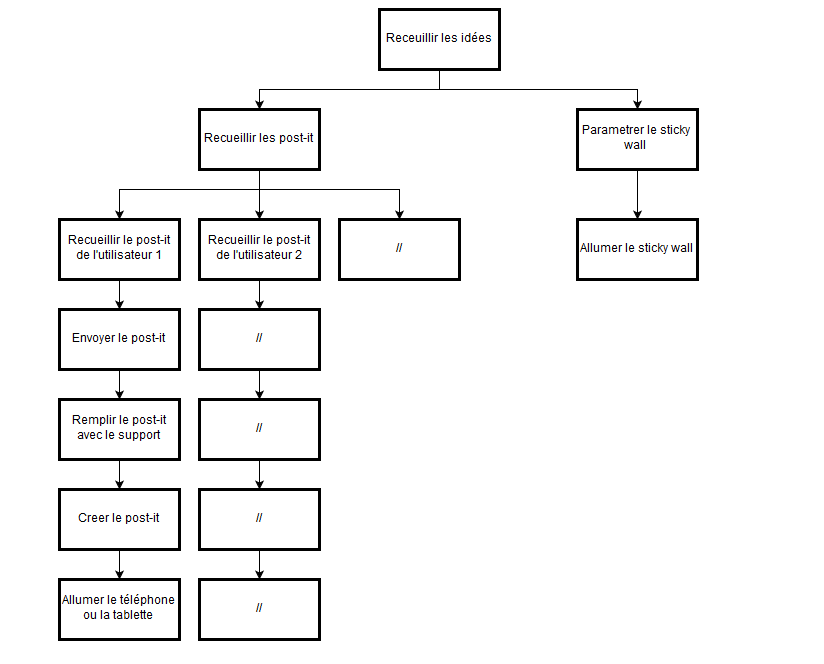
\includegraphics[width=\textwidth]{5}\\
\vspace{0.2cm}
\end{document}